% Conceptual schematic, not an execution trace or measured switching policy.
% Connected-route support and deferred delivery are distinct contracts.
\usetikzlibrary{arrows.meta}
\definecolor{routeink}{RGB}{35,105,112}
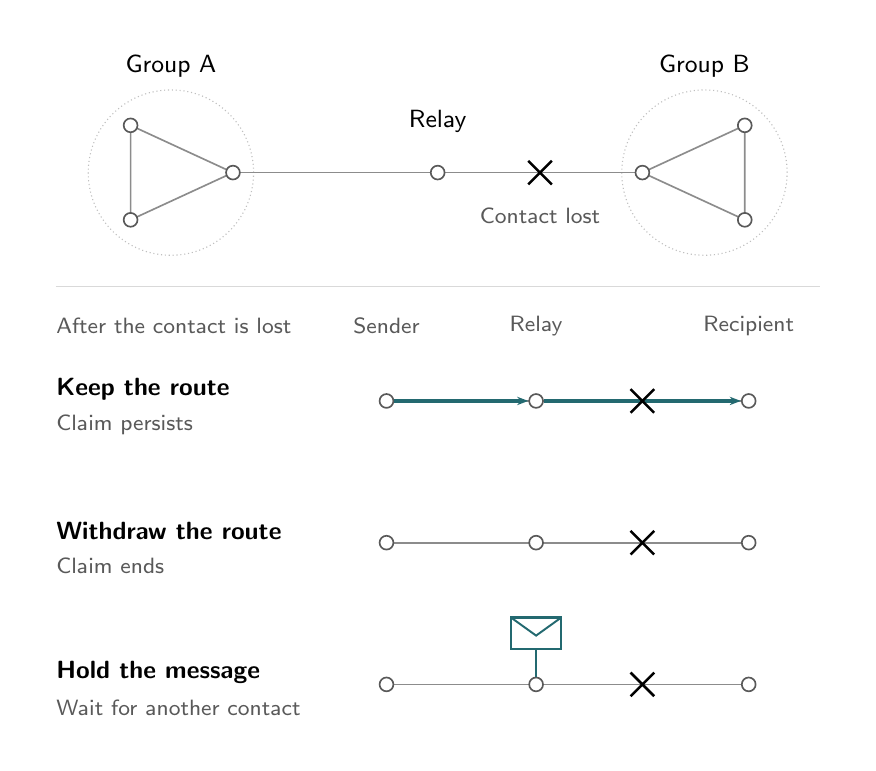
\begin{tikzpicture}[
  x=1cm,y=1cm,
  >={Stealth[length=4pt,width=3pt]},
  every node/.style={font=\sffamily\small,inner sep=0pt},
  device/.style={circle,draw=black!65,fill=white,line width=.6pt,minimum size=5pt},
  link/.style={draw=black!45,line width=.6pt},
  claim/.style={draw=routeink,line width=1.3pt,->},
  heading/.style={anchor=west,font=\sffamily\bfseries\small},
  note/.style={anchor=west,text=black!65,font=\sffamily\footnotesize}
]
% Two groups share a relay. Its contact with the right group disappears.
% Align the network's center (5.2) with the full figure's center (4.85).
\begin{scope}[xshift=-.35cm]
% Circumcenters give all three vertices equal clearance from each circle.
\draw[black!25,densely dotted] (1.812,7.5) ellipse (1.05 and 1.05);
\draw[black!25,densely dotted] (8.588,7.5) ellipse (1.05 and 1.05);
\node at (1.812,8.85) {Group A};
\node at (8.588,8.85) {Group B};
\node at (5.2,8.15) {Relay};
\draw[link] (1.3,8.1) -- (2.6,7.5) -- (1.3,6.9) -- cycle;
\draw[link] (7.8,7.5) -- (9.1,8.1) -- (9.1,6.9) -- cycle;
\draw[link] (2.6,7.5) -- (5.2,7.5) -- (7.8,7.5);
\draw[line width=.9pt] (6.35,7.65) -- (6.65,7.35)
                         (6.35,7.35) -- (6.65,7.65);
\node[text=black!65,font=\sffamily\footnotesize] at (6.5,6.95) {Contact lost};
\foreach \x/\y in {1.3/8.1,2.6/7.5,1.3/6.9,5.2/7.5,7.8/7.5,9.1/8.1,9.1/6.9} {
  \node[device] at (\x,\y) {};
}
\end{scope}

\draw[black!15] (0,6.05) -- (9.7,6.05);
\node[note] at (0,5.55) {After the contact is lost};
\foreach \x/\label in {4.2/Sender,6.1/Relay,8.8/Recipient} {
  \node[text=black!65,font=\sffamily\footnotesize] at (\x,5.55) {\label};
}

% The physical support is identical in all three rows.
\foreach \y in {4.6,2.8,1} {
  \draw[link] (4.2,\y) -- (6.1,\y) -- (8.8,\y);
  \foreach \x in {4.2,6.1,8.8} {\node[device] at (\x,\y) {};}
}

\node[heading] at (0,4.75) {Keep the route};
\node[note] at (0,4.3) {Claim persists};
\draw[claim] (4.3,4.6) -- (6,4.6);
\draw[claim] (6.2,4.6) -- (8.7,4.6);

\node[heading] at (0,2.95) {Withdraw the route};
\node[note] at (0,2.5) {Claim ends};

\node[heading] at (0,1.15) {Hold the message};
\node[note] at (0,.7) {Wait for another contact};
% An envelope at the relay represents retained message storage.
\draw[routeink,line width=.7pt] (6.1,1.1) -- (6.1,1.45);
\draw[routeink,fill=white,line width=.8pt] (5.78,1.45) rectangle (6.42,1.85);
\draw[routeink,line width=.7pt] (5.78,1.85) -- (6.1,1.62) -- (6.42,1.85);

% The same cross marks the missing physical contact in each response.
\foreach \y in {4.6,2.8,1} {
  \draw[line width=.9pt] (7.3,{\y+.15}) -- (7.6,{\y-.15})
                         (7.3,{\y-.15}) -- (7.6,{\y+.15});
}
\path (current bounding box.south west) ++(-.35,-.35)
  rectangle ([xshift=.35cm,yshift=.35cm]current bounding box.north east);
\end{tikzpicture}
